\begin{frame}{Heated cavity test case\footnote[frame,1]{Non-parametric study.}}
	\textbf{Stationary incompressible Navier-Stokes equations (with buoyancy and gravity):}

	We consider \only<1>{$\Omega = [-1,1]^2$ a squared domain}\only<2>{\textcolor{darkred}{$\bm{x}=(x,y)\in\Omega$}} and $\bm{e}_y = (0,1)$.
	
	Find \only<1>{the velocity $\bm{u}=(u_1,u_2)$, the pressure $p$ and the temperature $T$}\only<2>{\textcolor{darkred}{$\bm{U} = (\bm{u},p,T) = (u_1,u_2,p,T)$}} such that
	\begin{equation} \label{eq:Pb}
		\left\{\begin{aligned}
			&\only<1>{(\bm{u} \cdot \nabla)\bm{u} + \nabla p - \nu \Delta \bm{u} - g (\beta T + 1)\bm{e}_y}\only<2>{\textcolor{darkred}{R_{mom}(U;\bm{x},\bm{\mu})}} = 0 \;\; \text{in } \Omega \quad &&\text{\small (momentum)} \\
			&\only<1>{\nabla \cdot \bm{u}}\only<2>{\textcolor{darkred}{R_{inc}(U;\bm{x},\bm{\mu})}} = 0 \;\; \text{in } \Omega \quad &&\text{\small (incompressibility)} \\
			&\only<1>{\bm{u} \cdot \nabla T - k_f \Delta T}\only<2>{\textcolor{darkred}{R_{ener}(U;\bm{x},\bm{\mu})}} = 0 \;\; \text{in } \Omega \quad &&\text{\small (energy)} \only<1>{\\
			&\text{+ suitable BC}}
		\end{aligned}\right.
		\tag{$\mathcal{P}$}
	\end{equation}
	
	with $g=9.81$ the gravity, $\beta=0.1$ the expansion coefficient, $\nu=0.01$ the viscosity and $k_f=0.01$ the thermal conductivity. \only<1>{(Rayleigh number: \textcolor{darkred}{$156\,960$})}
    \only<2>{(Rayleigh number: $156\,960$)}

	\vspace{5pt}
	

	\uncover<2>{\textcolor{darkred}{\textbf{Boundary Conditions:}}

	\textbf{No-slip BC :} $\bm{u} = 0$ on $\partial\Omega$ \qquad \textbf{Isothermal BC :} $T = 1$ on the left wall ($x=-1$)\\
	\hspace{180pt}$T = -1$ on the right wall ($x=1$) \\
	\textbf{Adiabatic BC :} $\displaystyle \frac{\partial T}{\partial n} = 0$ on the top and bottom walls ($y=\pm 1$, denoted by $\Gamma_\text{ad}$)
    \vspace{5pt}
    }
\end{frame}

% \begin{frame}{Reference solution\footnote[frame,1]{Computed on an over-refined mesh ($h=7.10^{-3}$) on a $\mathbb{P}_3^2\times \mathbb{P}_2 \times \mathbb{P}_3$ continuous Lagrange FE space.}}
% 	\vspace{3pt}
% 	$\hspace{32pt} u_{1,\text{ref}} \hspace{67pt} u_{2,\text{ref}} \hspace{67pt} p_\text{ref} \hspace{67pt} T_\text{ref}$
% 	\vspace{-3pt}
    
% 	\begin{center}
% 		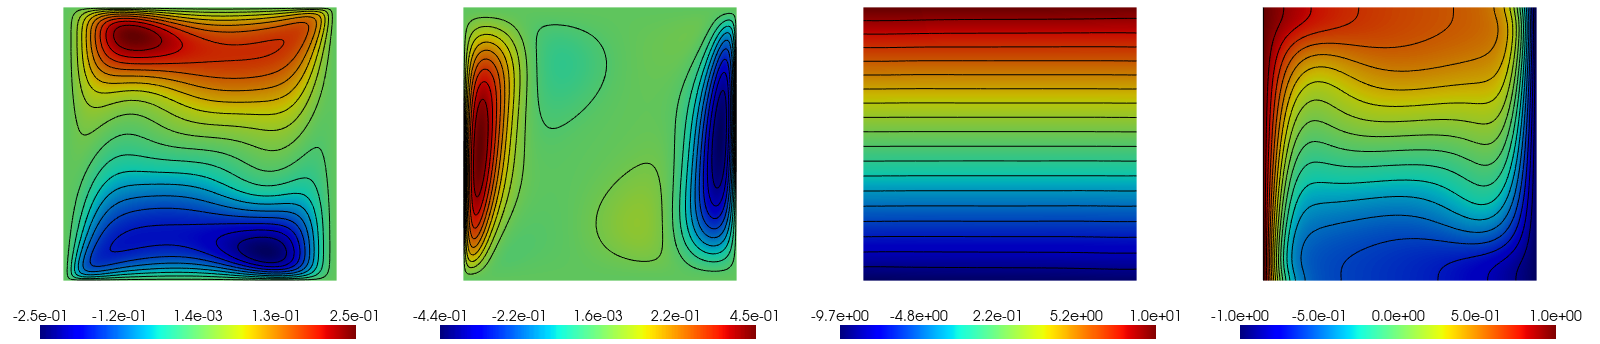
\includegraphics[width=0.98\linewidth]{images/nonlinear/uref3.png}
        
%         \vspace{5pt}
%         Rayleigh number : \textcolor{darkred}{$Ra = 156\,960$}

%         \vspace{5pt}
%         Strong natural convection with the presence of two counter-rotating vortices.
% 	\end{center}
% \end{frame}

\subsection[PINN]{Physics-Informed Neural Network (PINN)}

\begin{frame}{Neural Network considered}
    \vspace{-2pt}
    We consider a non-parametric NN with 2 inputs and 4 outputs, defined by
    $$U_\theta(\bm{x}) = \big(u_{1,\theta},u_{2,\theta},p_\theta,T_\theta)(\bm{x}).$$
    
    The Dirichlet boundary conditions are imposed on the outputs of the MLP by a \textbf{post-processing} step. \citep{Sukumar_2022}
    
    \begin{center}
        
\includegraphics[width=0.85\linewidth]{images/nonlinear/network/network.pdf}
    \end{center}

    \vspace{-5pt}
    We consider two levelsets functions $\varphi_1$ and $\varphi_2$, and the linear function $g$ defined by
    \begin{equation*}
        \varphi_1(x,y) = (x-1)(x+1)(y-1)(y+1),
    \end{equation*}
    \begin{equation*}
        \varphi_2(x,y) = (x-1)(x+1) \quad \text{and} \quad g(x,y) = 1 - (x+1).
    \end{equation*}
\end{frame}

\begin{frame}{PINN training}
    \vspace{-4pt}
    \textbf{Approximate the solution of \eqref{eq:Pb} by a PINN :} Find the optimal weights $\theta^\star$, such that
	
    \vspace{-8pt}
    \begin{equation}
		\label{eq:opt_pb_nl}
		\theta^\star = \argmin_{\theta}	\big( \; \textcolor{orange}{J_{inc}(\theta)} + \textcolor{orange}{J_{mom}(\theta)} + \textcolor{orange}{J_{ener}(\theta)} + \textcolor{darkred}{J_{ad}(\theta)} \; \big),
		\tag{$\mathcal{P}_\theta$}
	\end{equation}

    \vspace{-2pt}
	where the different cost functions\footnote[frame,1]{Discretized by a random process using Monte-Carlo method.} are defined by
	\vspace{5pt}

	\begin{minipage}{0.24\linewidth}
		\centering
		\textcolor{darkred}{adiabatic condition}
        
		\vspace{12pt}
		\textcolor{orange}{$3$ residual losses}
	\end{minipage}
	\begin{minipage}{0.68\linewidth}
		\centering
        \fcolorbox{darkred}{white}{
            $J_{ad}(\theta) =
            \int_{\mathcal{M}}\int_{\Gamma_\text{ad}} \big| \frac{\partial T_\theta(\bm{x},\bm{\mu})}{\partial n} \big|^2 d\bm{x} d\bm{\mu},$}
        
        \vspace{3pt}
		\fcolorbox{orange}{white}{
            $J_{\textbullet}(\theta) =
                \int_{\mathcal{M}}\int_{\Omega}
                \big| R_{\textbullet}(U_\theta(\bm{x},\bm{\mu});\bm{x},\bm{\mu}) \big|^2 d\bm{x} d\bm{\mu},$}
	\end{minipage}
    
    \vspace{5pt}
    with $U_\theta$ the non-parametric NN and $\textbullet$ the PDE considered (i.e. $inc$, $mom$ or $ener$).

    \vspace{-7pt}
    \vspace{3pt}    
    \begin{center}
        \begin{minipage}{0.62\linewidth}
            \centering
            \vspace{-8pt}
            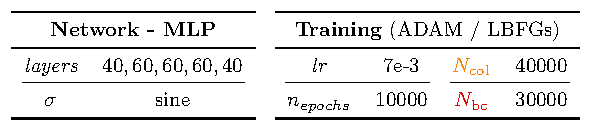
\includegraphics[width=0.94\linewidth]{images/nonlinear/training_param/training_param.pdf}

            \small\vspace{-3pt}
            + some weights to balance the different losses.
        \end{minipage}
        \begin{minipage}{0.36\linewidth}
            \centering
            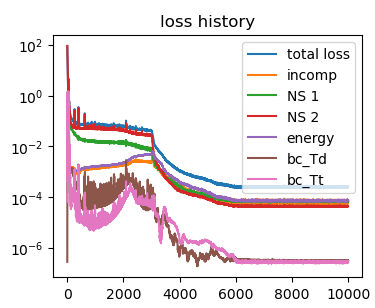
\includegraphics[width=0.84\linewidth]{images/nonlinear/training/test4_v3.png}
        \end{minipage}
    \end{center}
    
    \vspace{-8pt}
\end{frame}

\begin{frame}{Non parametric PINN prediction}
    \vspace{-4pt}
    \textbf{Prediction:} \begin{minipage}{0.26\linewidth}
        \centering
        $u_{1,\theta}$ \\
        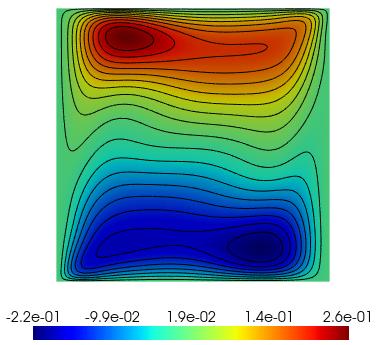
\includegraphics[width=0.95\linewidth]{images/nonlinear/PINN_param3_v3/PINN_plot_case4_v3_param1_u1.png}
    \end{minipage} \; \begin{minipage}{0.26\linewidth}
        \centering
        $u_{2,\theta}$ \\
        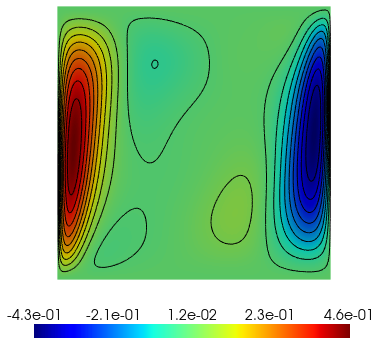
\includegraphics[width=0.95\linewidth]{images/nonlinear/PINN_param3_v3/PINN_plot_case4_v3_param1_u2.png}
    \end{minipage} \; \begin{minipage}{0.26\linewidth}
        \centering
        $T_\theta$ \\
        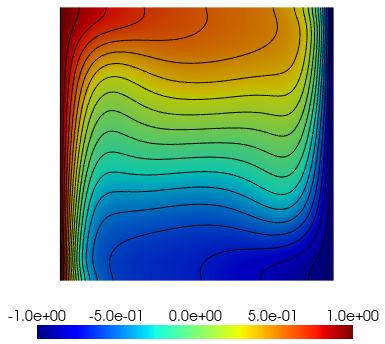
\includegraphics[width=0.95\linewidth]{images/nonlinear/PINN_param3_v3/PINN_plot_case4_v3_param1_T.png}
    \end{minipage}

    % \vspace{8pt}

    \textbf{Error map\footnote[frame,1]{Reference solution computed by FEM on an over-refined mesh.}:} \begin{minipage}{0.26\linewidth}
        \centering
        $u_{1,\text{ref}}-u_{1,\theta}$ \\
        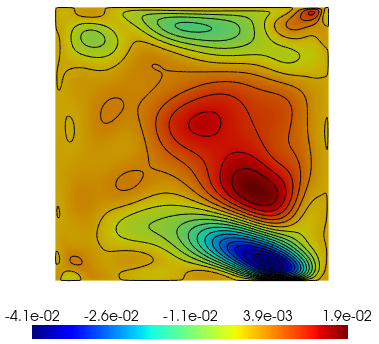
\includegraphics[width=0.95\linewidth]{images/nonlinear/PINN_param3_v3/PINN_error_plot_case4_v3_param1_u1.png}
    \end{minipage} \; \begin{minipage}{0.26\linewidth}
        \centering
        $u_{2,\text{ref}}-u_{2,\theta}$ \\
        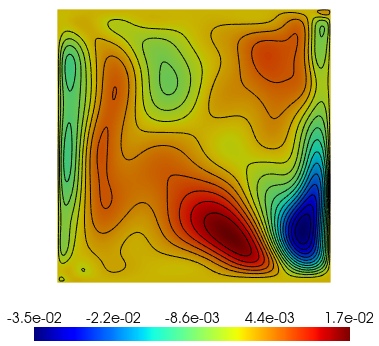
\includegraphics[width=0.95\linewidth]{images/nonlinear/PINN_param3_v3/PINN_error_plot_case4_v3_param1_u2.png}
    \end{minipage} \; \begin{minipage}{0.26\linewidth}
        \centering
        $T_\text{ref}-T_\theta$ \\
        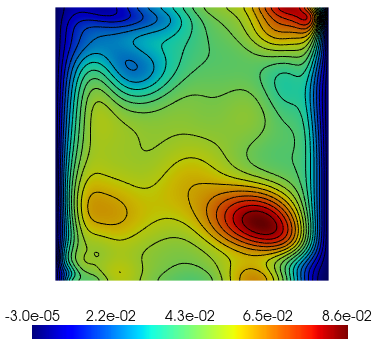
\includegraphics[width=0.95\linewidth]{images/nonlinear/PINN_param3_v3/PINN_error_plot_case4_v3_param1_T.png}
    \end{minipage}
    
    \vspace{-8pt}
    \textbf{$L^2$ error:} \\
    \textbf{\small (relative)} \hspace{25pt} $7.60\times10^{-2} \hspace{42pt} 5.38\times10^{-2} \hspace{42pt}  9.63\times10^{-2}$

    \vspace{10pt}
\end{frame}